% ISI manuscript draft -- journal-neutral article class; switch to the target journal's template at submission.
% Numbers marked \TBD{...} come from the converged Meep runs (isi/colab notebook) and must be filled in.
\documentclass[11pt,a4paper]{article}
\usepackage[margin=2.4cm]{geometry}
\usepackage{amsmath,amssymb,graphicx,booktabs,siunitx,xcolor}
\usepackage[colorlinks=true,linkcolor=blue!50!black,citecolor=blue!50!black,urlcolor=blue!50!black]{hyperref}
\usepackage[numbers,sort&compress]{natbib}
\usepackage{authblk}
\newcommand{\TBD}[1]{\textcolor{red}{\textbf{[#1]}}}
\newcommand{\Fp}{F_p}
\sisetup{range-phrase=--,range-units=single}
\graphicspath{{../figures/}}

\title{Resonant versus geometric anisotropy of the Purcell enhancement near a gold nanorod:\\
an equal-volume-sphere control and design rules for plasmon-enhanced single-photon sources}
\author[1]{Amin Hossein Sadidi}
\author[1]{Seyed Mohammad Parsa Molaei Tabari}
\author[1]{Malek Bagheri Harouni\thanks{Corresponding author: \TBD{e-mail}}}
\affil[1]{Department of Physics, Faculty of Science, University of Isfahan, Isfahan, Iran}
\date{}

\begin{document}
\maketitle

\begin{abstract}
The decay rate of a quantum emitter near a metal nanoparticle is governed by the projected local density of
optical states, and near an elongated particle this quantity depends strongly on the emitter's orientation.
How much of that orientational anisotropy is a generic near-surface effect, present for any metal body, and how
much is specific to the resonant longitudinal mode of the elongated particle, has not been separated
quantitatively. We address this question for a dipole \SI{5}{nm} from the tip of a capped gold nanorod
(length \SI{60}{nm}, diameter \SI{20}{nm}) using three-dimensional finite-difference time-domain simulations,
validated against exact Mie theory, and a set of controls: free space, a transverse dipole at the same tip,
and an equal-volume gold sphere probed with radial and tangential dipoles. The longitudinal dipole reaches a
Purcell factor $\Fp\approx\num{1.5e3}$ at \SI{610}{nm} and a radiative enhancement $T\approx\num{1.2e2}$ at
\SI{616}{nm}, but more than \SI{92}{\percent} of the emitted power is absorbed in the metal. The sphere's
radial-to-tangential ratio stays between 2.2 and 2.7 over the whole \SIrange{500}{900}{nm} band, consistent
with the quasi-static near-surface limit of 2, and the nanorod shows the same ratio away from resonance; at
the longitudinal resonance the nanorod ratio rises to 41 for $\Fp$ and to 358 for $T$. The orientational
anisotropy of the nanorod is therefore predominantly resonant, and it is removed by any scalar or
orientation-averaged description. Including the intrinsic quantum yield $q_0$ of the emitter, we find that
the optimal tip--emitter gap depends on $q_0$: for poor emitters ($q_0=0.01$) a \SIrange{5}{10}{nm} gap raises
the quantum efficiency eightfold, whereas for $q_0\to1$ the \SI{20}{nm} gap performs best. Mesh-convergence
analysis with a body-of-revolution solver gives peak values converged to \TBD{x\,\%}.
\end{abstract}

\noindent\textbf{Keywords:} Purcell effect; local density of optical states; gold nanorod; plasmonic nanoantenna;
quenching; single-photon source; FDTD.

% ---------------------------------------------------------------------------------------------
\section{Introduction}

The spontaneous emission rate of a quantum emitter is not an intrinsic property but depends on its
electromagnetic environment~\cite{purcell,novotny}. Metallic nanoparticles supporting localized surface plasmon
resonances confine light to volumes far below the diffraction limit and can enhance emission rates by several
orders of magnitude~\cite{maier,vanhulst,bharadwaj2009}. This has made plasmonic nanoantennas a candidate
platform for bright, fast single-photon sources~\cite{koenderink,hoang,akselrod,senellart}, in which a large
rate enhancement shortens the excited-state lifetime and raises the achievable repetition rate, and a short
radiative lifetime relative to the dephasing time is a prerequisite for indistinguishable photons~\cite{aharonovich}.

The price of plasmonic confinement is absorption. At emitter--metal separations of a few nanometres, energy is
transferred to non-radiative channels in the metal, and the fluorescence is quenched rather than
enhanced~\cite{anger,kuhn,ford,carminati2006}. The total decay rate and the radiative rate therefore have to be
treated separately, and their ratio---the antenna quantum efficiency---depends sensitively on distance,
wavelength and the intrinsic quantum yield of the emitter~\cite{bharadwaj2007,khurgin}.

Gold nanorods are attractive antennas because their longitudinal plasmon resonance is tunable through the
aspect ratio across the visible and near infrared~\cite{chen,sonnichsen}, they can be synthesised with good
control~\cite{nikoobakht}, and their tips concentrate the near field. Single-molecule experiments have
demonstrated fluorescence enhancements exceeding a thousandfold near individual gold nanorods~\cite{yuan,khatua},
and theory has established that the decay-rate enhancement near the tip reaches the order of $10^3$ while the
efficiency falls in nanometre gaps~\cite{mohammadi}.

A consequence of the nanorod's elongated shape is a strong dependence of the response on the orientation of the
emitter's transition dipole. In the language of Eq.~\eqref{eq:ldos}, the Green tensor at the emitter position is
anisotropic, and the decay rate is the projection of that tensor on the dipole direction~\cite{novotny}. Yet a
dipole close to any metal surface---a sphere or a plane---also shows an orientation dependence, because the
image dipole of a perpendicular dipole adds in phase whereas that of a parallel dipole subtracts; in the
quasi-static limit the ratio of perpendicular to parallel decay rates near a surface tends to two~\cite{ford}. It
is therefore not obvious how much of the anisotropy observed near a nanorod tip is generic and how much is caused
by the longitudinal resonance that distinguishes the nanorod from a compact particle. This distinction matters
in practice: emitters such as colloidal quantum dots or dye molecules are often randomly oriented, and
orientation-averaged or scalar descriptions---for example a single ``Purcell factor''---discard precisely the
resonant part.

In this work we separate the two contributions quantitatively by introducing an equal-volume gold sphere as a
control and probing both the nanorod and the sphere with two dipole orientations at an identical gap. We
further include free-space normalisation, analytic Mie validation, a gap sweep and a mesh-convergence study, and
we translate the results into design rules for plasmon-enhanced single-photon sources that account for the
intrinsic quantum yield of the emitter and the collection numerical aperture.

% ---------------------------------------------------------------------------------------------
\section{Theory}

For a point dipole $\mathbf{p}=p\,\hat{\mathbf n}$ at $\mathbf r_0$ in the weak-coupling regime, the total decay
rate normalised to its free-space value is~\cite{novotny}
\begin{equation}
  \frac{\Gamma_{\rm tot}}{\Gamma_0} = \frac{6\pi c}{\omega}\,
  \hat{\mathbf n}\cdot\mathrm{Im}\,\overleftrightarrow{\mathbf G}(\mathbf r_0,\mathbf r_0;\omega)\cdot\hat{\mathbf n}
  \equiv \Fp(\omega),
  \label{eq:ldos}
\end{equation}
where $\overleftrightarrow{\mathbf G}$ is the dyadic Green function. Classically, $\Fp=P_{\rm tot}/P_0$ is the
power delivered by a constant-amplitude dipole relative to free space, which is how it is evaluated
numerically below. The power radiated to the far field, $T=P_{\rm rad}/P_0$, gives the radiative enhancement,
and the difference $\Fp-T=P_{\rm loss}/P_0$ is absorbed in the metal. For an emitter of intrinsic quantum yield
$q_0$, the quantum efficiency in the presence of the antenna is~\cite{bharadwaj2007}
\begin{equation}
  \eta(q_0) = \frac{T}{\Fp + (1-q_0)/q_0},
  \label{eq:eta}
\end{equation}
which reduces to the antenna efficiency $\eta_a=T/\Fp$ for $q_0=1$.

The orientation average $\tfrac13\mathrm{Tr}\,\mathrm{Im}\,\overleftrightarrow{\mathbf G}$ equals the projected
value only for an isotropic Green tensor. For a dipole on the symmetry axis of a body of revolution, the tensor is
diagonal with an axial component $G_{zz}$ and a transverse component $G_{xx}=G_{yy}$; the anisotropy is
fully characterised by the ratio $\Fp^{\parallel{\rm axis}}/\Fp^{\perp{\rm axis}}$. We define the analogous ratio
for the radiative channel, $T^{\parallel}/T^{\perp}$. For a sphere, axial and transverse correspond to radial
and tangential dipoles, for which exact Mie expressions exist~\cite{ruppin,kim,mertens}. The equal-volume sphere
thus provides a reference in which only the generic near-surface anisotropy is present: it has the same
amount of gold, the same dipole--surface gap, but no elongated resonance.

% ---------------------------------------------------------------------------------------------
\section{Methods}

\subsection{Geometry and cases}
The nanorod is a gold cylinder of length \SI{40}{nm} and radius $R=\SI{10}{nm}$ terminated by two hemispherical
caps (total length $L=\SI{60}{nm}$, aspect ratio 3), a geometry accessible by seed-mediated
growth~\cite{nikoobakht}. The dipole is placed on the rod axis at a distance $d$ from the apex ($d=\SI{5}{nm}$
unless stated otherwise). The equal-volume sphere has $R_{\rm sph}=\SI{15.874}{nm}$
($\tfrac43\pi R_{\rm sph}^3=\pi R^2\cdot\SI{40}{nm}+\tfrac43\pi R^3$). The cases are: A, rod with axial
(longitudinal) dipole; C, rod with transverse dipole; D and D$_\perp$, sphere with radial and tangential dipoles;
B, free space; plus gap (3--\SI{20}{nm}) and mesh variations of case~A. The host is air unless stated.

\subsection{Gold permittivity}
We use the Johnson--Christy data~\cite{johnson}. For the time-domain solvers it is represented by a Drude term
plus two Lorentz poles fitted over \SIrange{440}{1000}{nm} (root-mean-square relative error \SI{1.6}{\percent},
maximum \SI{3.4}{\percent}); the fit parameters are given in the Supplementary Information. The same fitted
permittivity is used in the Mie reference calculations so that the comparison isolates discretisation errors.

\subsection{Numerical methods}
\emph{Full three-dimensional FDTD.} Cases A--D$_\perp$ were first computed with a commercial FDTD solver
(Lumerical FDTD 2024~R1)~\cite{taflove,lumerical} with a \SI{600}{nm} simulation domain, twelve PML layers, a
uniform \SI{2}{nm} override mesh around the particle and gap, and a \SI{400}{nm} closed box of power monitors.
$\Fp$ is obtained from the power injected by the dipole and $T$ from the flux through the box, both normalised
to the same dipole in a homogeneous medium.

\emph{Body-of-revolution FDTD.} Because the dipole lies on the symmetry axis, the fields can be expanded as
$e^{im\varphi}$ and an axial dipole couples only to $m=0$ and a transverse dipole only to $m=\pm1$. The
three-dimensional problem then reduces to a two-dimensional one in the $(r,z)$ half-plane without approximation.
We exploit this with the open-source solver Meep~\cite{meep} in cylindrical coordinates, which allows grid
spacings down to \TBD{0.5}\,nm. $\Fp$ is computed from the local density of states at the dipole, $T$ from the
flux through a closed surface around the particle, and the angular emission pattern from a near-to-far-field
transformation, from which the fraction of radiated power collected within a numerical aperture NA is obtained.
To avoid normalisation errors at the edges of a broadband pulse, the \SIrange{490}{910}{nm} band is covered by
three overlapping sub-band simulations of which only the central parts are retained.

\subsection{Validation}
For case D, the exact Mie solution~\cite{ruppin,kim} gives $\Fp=772$ at \SI{506}{nm} and $T=6.58$ at
\SI{530}{nm}. The \SI{2}{nm}-mesh three-dimensional FDTD reproduces both peak positions within \SI{2}{nm} but
underestimates the peak heights by \SI{15}{\percent} and \SI{8}{\percent} (Fig.~\ref{fig:mie}). The
body-of-revolution solver reproduces the Mie result for a dielectric sphere to within \SI{1}{\percent} in the
centre of each sub-band at a \SI{2}{nm} grid, and for gold to within \TBD{x\,\%} at \TBD{0.5}\,nm
(Supplementary Information). The free-space reference yields $\Fp^{B}$ between 0.93 and 1.13 and $T^{B}$
between 0.993 and 1.003 in the three-dimensional solver, which bounds the normalisation uncertainty of the
three-dimensional results.

% ---------------------------------------------------------------------------------------------
\section{Results}

\subsection{Total and radiative enhancement of the axial dipole}
Figure~\ref{fig:spectra} shows $\Fp$, $T$ and $\eta_a$ for cases A, C and D. For the axial dipole at the rod tip
(case~A), $\Fp$ peaks at \num{1.50e3} at \SI{610}{nm} and $T$ at 119 at \SI{616}{nm}. The radiative peak is red
shifted by \SI{6}{nm} relative to the Purcell peak, because $\Fp$ contains higher-order, non-radiative multipoles
that lie to the blue of the dipolar mode whereas $T$ is dominated by the dipolar mode~\cite{anger,bharadwaj2007}.
At the Purcell peak $\eta_a=\SI{7.6}{\percent}$, i.e.\ $P_{\rm loss}/P_0=\Fp-T=1383$ and more than
\SI{92}{\percent} of the emitted energy is absorbed. The highest efficiency, \SI{19}{\percent}, is reached at
\SI{784}{nm}, far from resonance, where $\Fp$ has dropped to 69. A second, weaker $\Fp$ maximum at
\SI{512}{nm} ($\Fp=645$, $T\approx1.8$) coincides with the onset of interband absorption in gold and is almost
purely non-radiative. These magnitudes agree with earlier calculations for comparable rods and
gaps~\cite{mohammadi}. The mesh-converged body-of-revolution values are $\Fp=\TBD{x}$ at \TBD{x}\,nm and
$T=\TBD{x}$ at \TBD{x}\,nm.

\subsection{Orientation anisotropy: nanorod versus equal-volume sphere}
Rotating the dipole to the transverse direction at the same position (case C) reduces $\Fp$ at \SI{610}{nm}
by a factor of 41 and $T$ at \SI{616}{nm} by a factor of 358. The transverse dipole radiates even less than in free
space ($T_{\max}=0.48$) and its own $\Fp$ maximum (239 at \SI{508}{nm}) reflects absorption near the interband
edge rather than a radiative resonance.

The equal-volume sphere answers whether this anisotropy is specific to the rod (Fig.~\ref{fig:orientation}).
For the sphere, the radial-to-tangential ratio of $\Fp$ lies between 2.2 and 2.7 throughout
\SIrange{500}{900}{nm}, close to the quasi-static near-surface value of two~\cite{ford}, and shows no resonant
structure. For the nanorod, the same ratio is 2.6--2.8 below the resonance (\SIrange{500}{530}{nm})---the
sphere value---but rises steeply to 41 at the longitudinal resonance. The radiative ratio behaves alike:
\numrange{10}{50} for the sphere, from about 4 off resonance to 358 on resonance for the rod.

The anisotropy of the nanorod Green tensor therefore splits into two contributions: a geometric,
near-surface factor of order two that any metal body produces, and a resonant factor of order
\numrange{10}{e2} that belongs exclusively to the longitudinal ($m=0$) mode of the elongated particle. A scalar
or orientation-averaged description removes the second contribution entirely. The comparison with the sphere at
equal volume further shows that the enhancement near \SI{610}{nm} is not a volume effect: there the rod exceeds the
sphere by factors of 15.6 in $\Fp$ and 24 in $T$, while at their respective maxima the ratios are 2.3 and 20.

\subsection{Gap dependence and the enhancement--efficiency trade-off}
Increasing the gap from 5 to 10 and \SI{20}{nm} (Fig.~\ref{fig:gap}) leaves the radiative peak at
\SIrange{614}{618}{nm} while $\Fp$ falls from \num{1496} to 553 and 91 and $T$ from 119 to 47 and 9.9. The antenna
efficiency at the radiative peak increases only modestly (\SI{8.6}{\percent}, \SI{8.9}{\percent},
\SI{12}{\percent}), whereas its spectral maximum rises from \SI{19}{\percent} to \SI{31}{\percent} and
\SI{74}{\percent}. The exact solution for the sphere (Fig.~\ref{fig:gap}, lower row) shows the same trade-off,
which is generic for nanometre gaps~\cite{alhamadani}. At \SI{3}{nm} the peak $\Fp$ (\num{7198} at \SI{516}{nm},
computed with a \SI{1}{nm} mesh) is entirely non-radiative ($\eta_a=\SI{0.05}{\percent}$); at this distance
surface scattering, $\gamma=\gamma_{\rm bulk}+Av_F/R$~\cite{kreibig,coronado}, and nonlocal response~\cite{ciraci,mortensen}
become significant, and quasinormal-mode treatments~\cite{sauvan,lalanne} are required to relate the LDOS to
modal Purcell factors.

\subsection{Design rule: the optimal gap depends on the emitter's intrinsic quantum yield}
For single-photon sources the relevant figure of merit depends on the operating regime. If the repetition rate is
limited by the emitter, the photon rate scales with $T=\Fp\eta_a$; in the common situation that a pulsed laser
sets the repetition rate and the lifetime is already much shorter than the pulse period, the number of photons
per pulse scales with $\eta$ of Eq.~\eqref{eq:eta}~\cite{koenderink,hoang}. Figure~\ref{fig:q0} and
Table~\ref{tab:q0} evaluate $\eta(q_0)$ at the radiative peak for each gap. For an ideal emitter ($q_0=1$) the
\SI{20}{nm} gap is best (\SI{12.4}{\percent}) and the \SI{3}{nm} gap worst (\SI{6.4}{\percent}). For a poor emitter
($q_0=0.01$) the order is reversed in the range 5--\SI{20}{nm}: the \SI{5}{nm} and \SI{10}{nm} gaps raise the
efficiency from \SI{1}{\percent} to about \SI{8}{\percent}, while the \SI{20}{nm} gap gives \SI{5.5}{\percent}. The
crossover follows from Eq.~\eqref{eq:eta}: a large $\Fp$ is needed to outcompete the intrinsic non-radiative rate
$(1-q_0)/q_0$, but beyond that point additional $\Fp$ only feeds absorption. The optimal gap therefore increases
with $q_0$, and the design of a nanorod antenna cannot be separated from the photophysics of the emitter.

\begin{table}[t]\centering
\caption{Quantum efficiency $\eta(q_0)$ at the radiative peak of the rod (axial dipole), Eq.~\eqref{eq:eta}, from the
three-dimensional FDTD spectra. The 3-nm case used a 1-nm mesh, the others 2~nm.}\label{tab:q0}
\begin{tabular}{rrrrrrrr}\toprule
gap (nm) & $\lambda_T$ (nm) & $\Fp(\lambda_T)$ & $T_{\max}$ & $q_0=0.01$ & $0.1$ & $0.5$ & $1$\\\midrule
 3 & 614 & 3913 & 252 & 0.063 & 0.064 & 0.064 & 0.064\\
 5 & 616 & 1393 & 119 & 0.080 & 0.085 & 0.086 & 0.086\\
10 & 614 &  528 & 46.8 & 0.075 & 0.087 & 0.089 & 0.089\\
20 & 618 & 79.5 & 9.87 & 0.055 & 0.112 & 0.123 & 0.124\\\bottomrule
\end{tabular}
\end{table}

\subsection{Collection efficiency}
The axial dipole and the longitudinal mode radiate with a dipolar pattern oriented along the rod, which sets the
fraction of the radiated power that a lens can collect. \TBD{Fraction within NA = 0.9 / 1.3 from the
near-to-far-field transformation, gap and aspect-ratio maps in air and water.}

\subsection{Numerical accuracy}
In the three-dimensional solver, the resonance position (\SI{616 \pm 4}{nm}) and the efficiency at the radiative
peak are stable when the override mesh is changed between 3, 2 and \SI{1.5}{nm}, but the peak heights are not
monotonic (Fig.~S\TBD{x}): the peak $T$ is 184, 119 and 165, and at \SI{1.5}{nm} a spurious non-radiative feature
appears. The cause is the sub-cell position of the source in a \SI{5}{nm} gap together with the staircased
cap: with a non-radiative rate scaling as $d^{-3}$~\cite{ford,novotny}, a one-nanometre effective displacement
changes the loss channel by up to a factor of two. All ratios reported above are computed with an identical
mesh and source position and are insensitive to this error. The body-of-revolution solver, in which the
source lies exactly on the axis and the grid can be refined to \TBD{0.5}\,nm, gives converged peak values of
\TBD{x} with a residual change of \TBD{x\,\%} between the two finest grids.

% ---------------------------------------------------------------------------------------------
\section{Discussion}
The central result is that the strong orientation dependence of emission near a nanorod tip is mostly resonant.
For randomly oriented emitters, the orientation-averaged rate is
$\langle\Fp\rangle=(\Fp^{\parallel}+2\Fp^{\perp})/3$; at the resonance the axial contribution dominates and
$\langle\Fp\rangle\approx\Fp^{\parallel}/3$, but the averaged efficiency mixes a moderately efficient axial channel
with a strongly quenched transverse one. Experiments that report a single enhancement factor for an ensemble of
orientations~\cite{yuan,khatua} thus measure a quantity that depends on the orientation distribution, and our
decomposition indicates how to translate between them.

The equal-volume comparison also clarifies the role of shape. A compact particle of the same volume provides
only the near-surface factor of order two and a weak, interband-dominated response; the elongated geometry adds a
radiative resonance that is red shifted out of the interband region, where gold is less lossy. This is why the
rod's radiative enhancement exceeds the sphere's by an order of magnitude even though the metal volume is equal.

For single-photon sources, a short lifetime (large $\Fp$) and a high quantum efficiency are both required. Our
results show that a \SIrange{5}{10}{nm} gap is preferable for emitters with low intrinsic yield, such as many
colloidal quantum dots at room temperature, while near-unity emitters benefit more from larger gaps; tuning the
longitudinal resonance through the aspect ratio provides an independent handle on the emission wavelength.
\TBD{Collection-efficiency and aqueous-environment maps (Colab runs) to be summarised here.}

The limitations of the present study are the local-response description of gold, which is adequate at
\SI{5}{nm} but not in sub-nanometre gaps where tunnelling and nonlocality matter~\cite{xu,ciraci}; the
classical treatment of the emitter in the weak-coupling regime; and the restriction to on-axis emitters.

% ---------------------------------------------------------------------------------------------
\section{Conclusion}
Using a capped gold nanorod and an equal-volume sphere probed with two dipole orientations at the same gap, we
have separated the orientational anisotropy of the Purcell enhancement into a generic near-surface factor of
about two and a resonant factor of up to $10^2$ that is specific to the longitudinal mode. More than
\SI{92}{\percent} of the emitted power is absorbed at the Purcell maximum for a \SI{5}{nm} gap, and the optimal gap
for a single-photon source depends on the intrinsic quantum yield of the emitter. Simulation scripts, raw spectra
and analysis code are openly available.

\section*{Data availability}
All raw spectra, simulation scripts (Lumerical and Meep) and analysis code are available at
\TBD{Zenodo DOI / GitHub URL}.

\section*{Author contributions}
\TBD{to be completed by the authors.}

\section*{Conflict of interest}
The authors declare no competing interests.

% ---------------------------------------------------------------------------------------------
\begin{figure}[p]\centering
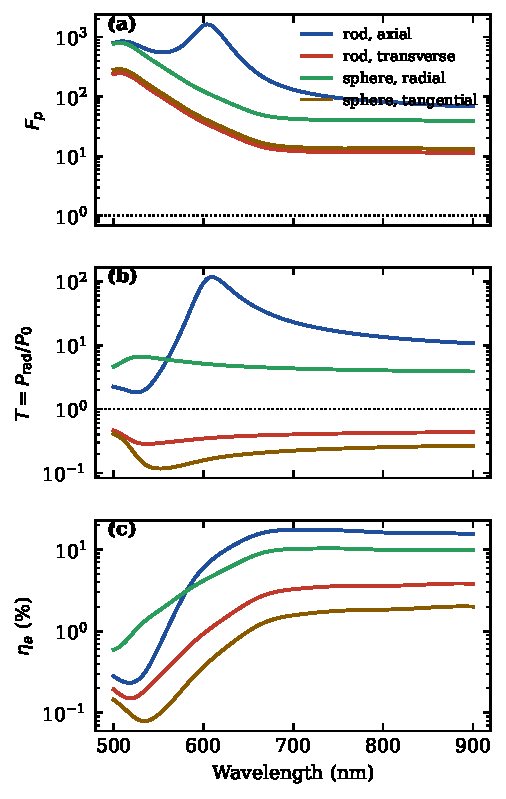
\includegraphics[width=0.55\linewidth]{fig_spectra.pdf}
\caption{(a) Purcell factor, (b) radiative enhancement and (c) antenna efficiency for the rod with axial (A) and
transverse (C) dipole and the equal-volume sphere with radial dipole (D), all at a \SI{5}{nm} gap; dotted: free-space
reference B. Dashed line: \SI{610}{nm}.}\label{fig:spectra}
\end{figure}
\begin{figure}[p]\centering
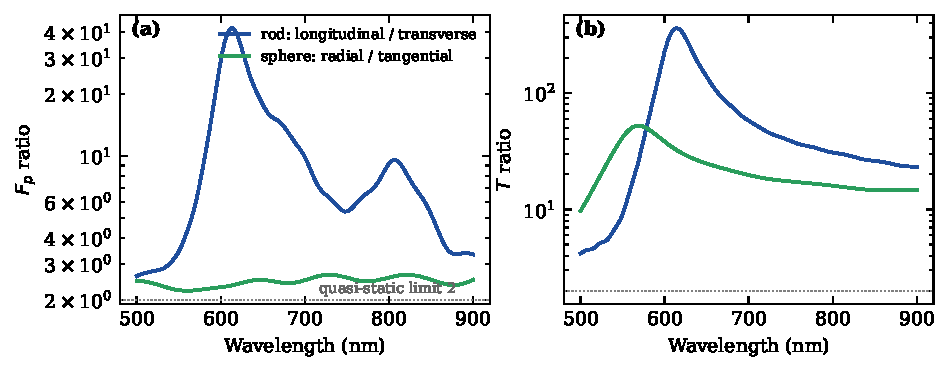
\includegraphics[width=\linewidth]{fig_orientation.pdf}
\caption{Orientation ratios of (a) $\Fp$ and (b) $T$ for the rod (axial/transverse) and the equal-volume sphere
(radial/tangential) at a \SI{5}{nm} gap. Dotted: quasi-static near-surface limit of 2.}\label{fig:orientation}
\end{figure}
\begin{figure}[p]\centering
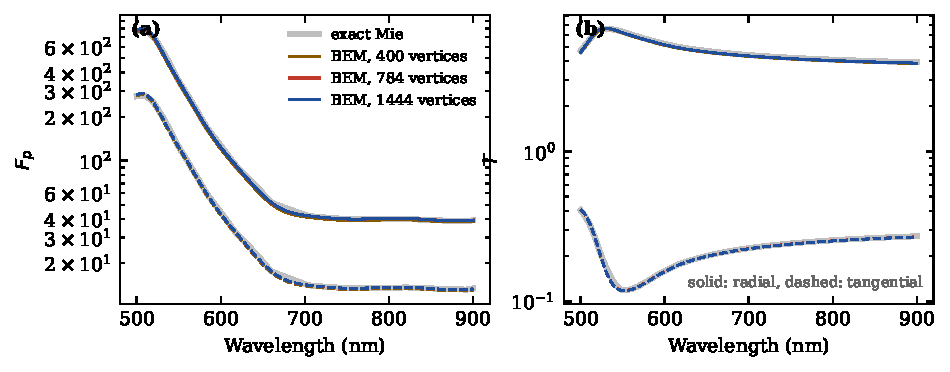
\includegraphics[width=0.55\linewidth]{fig_mie.pdf}
\caption{Validation against exact Mie theory for the equal-volume sphere with radial dipole at \SI{5}{nm}:
(a) $\Fp$, (b) $T$.}\label{fig:mie}
\end{figure}
\begin{figure}[p]\centering
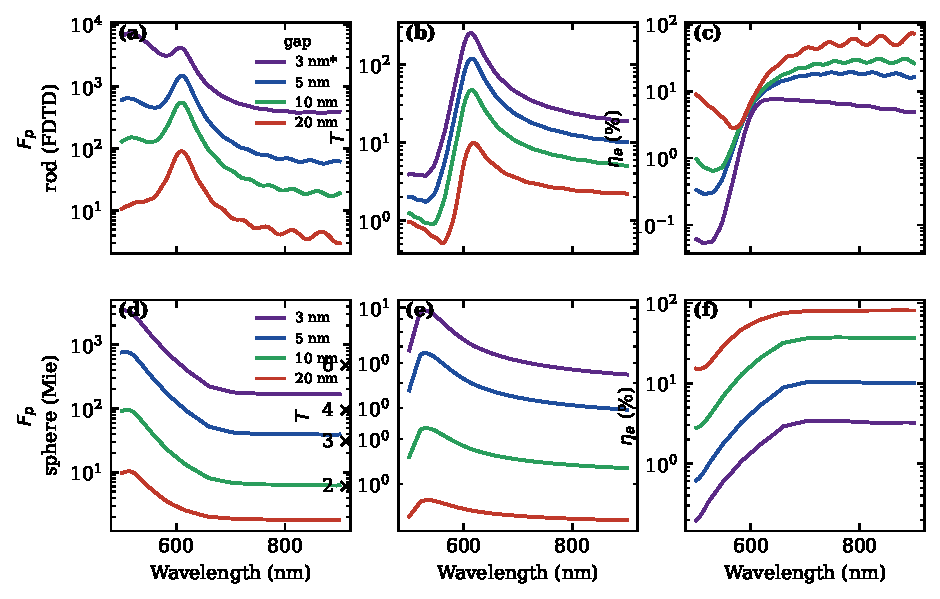
\includegraphics[width=\linewidth]{fig_gap.pdf}
\caption{Gap dependence of $\Fp$, $T$ and $\eta_a$ for the rod with axial dipole (top, FDTD; *1-nm mesh) and the
equal-volume sphere with radial dipole (bottom, exact Mie).}\label{fig:gap}
\end{figure}
\begin{figure}[p]\centering
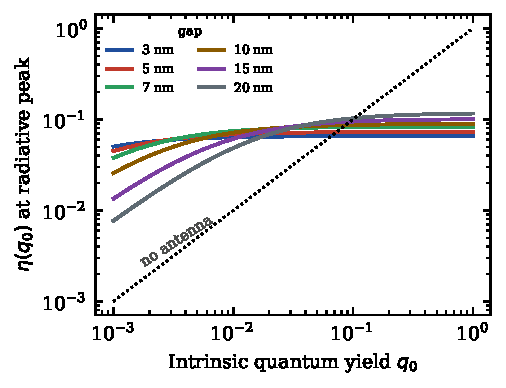
\includegraphics[width=0.55\linewidth]{fig_q0.pdf}
\caption{Quantum efficiency at the radiative peak versus intrinsic quantum yield, Eq.~\eqref{eq:eta}, for four
gaps. Dotted: emitter without antenna ($\eta=q_0$).}\label{fig:q0}
\end{figure}

\begin{thebibliography}{62}
\bibitem{purcell} Purcell E. M. Spontaneous emission probabilities at radio frequencies. \textit{Physical Review} \textbf{69}, 681 (1946). \href{https://doi.org/10.1103/PhysRev.69.674.2}{doi:10.1103/PhysRev.69.674.2}

\bibitem{novotny} Novotny L., Hecht B. \textit{Principles of Nano-Optics}, 2nd ed. Cambridge University Press, Cambridge (2012). \href{https://doi.org/10.1017/CBO9780511794193}{doi:10.1017/CBO9780511794193}

\bibitem{maier} Maier S. A. \textit{Plasmonics: Fundamentals and Applications}. Springer, New York (2007). \href{https://doi.org/10.1007/0-387-37825-1}{doi:10.1007/0-387-37825-1}

\bibitem{vanhulst} Novotny L., van Hulst N. Antennas for light. \textit{Nature Photonics} \textbf{5}, 83--90 (2011). \href{https://doi.org/10.1038/nphoton.2010.237}{doi:10.1038/nphoton.2010.237}

\bibitem{bharadwaj2009} Bharadwaj P., Deutsch B., Novotny L. Optical antennas. \textit{Advances in Optics and Photonics} \textbf{1}, 438--483 (2009). \href{https://doi.org/10.1364/AOP.1.000438}{doi:10.1364/AOP.1.000438}

\bibitem{koenderink} Koenderink A. F. Single-photon nanoantennas. \textit{ACS Photonics} \textbf{4}, 710--722 (2017). \href{https://doi.org/10.1021/acsphotonics.7b00061}{doi:10.1021/acsphotonics.7b00061}

\bibitem{hoang} Hoang T. B., Akselrod G. M., Mikkelsen M. H. Ultrafast room-temperature single photon emission from quantum dots coupled to plasmonic nanocavities. \textit{Nano Letters} \textbf{16}, 270--275 (2016). \href{https://doi.org/10.1021/acs.nanolett.5b03724}{doi:10.1021/acs.nanolett.5b03724}

\bibitem{akselrod} Akselrod G. M., Argyropoulos C., Hoang T. B., Ciracì C., Fang C., Huang J., Smith D. R., Mikkelsen M. H. Probing the mechanisms of large Purcell enhancement in plasmonic nanoantennas. \textit{Nature Photonics} \textbf{8}, 835--840 (2014). \href{https://doi.org/10.1038/nphoton.2014.228}{doi:10.1038/nphoton.2014.228}

\bibitem{senellart} Senellart P., Solomon G., White A. High-performance semiconductor quantum-dot single-photon sources. \textit{Nature Nanotechnology} \textbf{12}, 1026--1039 (2017). \href{https://doi.org/10.1038/nnano.2017.218}{doi:10.1038/nnano.2017.218}

\bibitem{aharonovich} Aharonovich I., Englund D., Toth M. Solid-state single-photon emitters. \textit{Nature Photonics} \textbf{10}, 631--641 (2016). \href{https://doi.org/10.1038/nphoton.2016.186}{doi:10.1038/nphoton.2016.186}

\bibitem{anger} Anger P., Bharadwaj P., Novotny L. Enhancement and quenching of single-molecule fluorescence. \textit{Physical Review Letters} \textbf{96}, 113002 (2006). \href{https://doi.org/10.1103/PhysRevLett.96.113002}{doi:10.1103/PhysRevLett.96.113002}

\bibitem{kuhn} Kühn S., Håkanson U., Rogobete L., Sandoghdar V. Enhancement of single-molecule fluorescence using a gold nanoparticle as an optical nanoantenna. \textit{Physical Review Letters} \textbf{97}, 017402 (2006). \href{https://doi.org/10.1103/PhysRevLett.97.017402}{doi:10.1103/PhysRevLett.97.017402}

\bibitem{ford} Ford G. W., Weber W. H. Electromagnetic interactions of molecules with metal surfaces. \textit{Physics Reports} \textbf{113}, 195--287 (1984). \href{https://doi.org/10.1016/0370-1573(84)90098-X}{doi:10.1016/0370-1573(84)90098-X}

\bibitem{carminati2006} Carminati R., Greffet J.-J., Henkel C., Vigoureux J. M. Radiative and non-radiative decay of a single molecule close to a metallic nanoparticle. \textit{Optics Communications} \textbf{261}, 368--375 (2006). \href{https://doi.org/10.1016/j.optcom.2005.12.009}{doi:10.1016/j.optcom.2005.12.009}

\bibitem{bharadwaj2007} Bharadwaj P., Novotny L. Spectral dependence of single molecule fluorescence enhancement. \textit{Optics Express} \textbf{15}, 14266--14274 (2007). \href{https://doi.org/10.1364/OE.15.014266}{doi:10.1364/OE.15.014266}

\bibitem{khurgin} Khurgin J. B. How to deal with the loss in plasmonics and metamaterials. \textit{Nature Nanotechnology} \textbf{10}, 2--6 (2015). \href{https://doi.org/10.1038/nnano.2014.310}{doi:10.1038/nnano.2014.310}

\bibitem{lu2020} Lu X., Ye G., Punj D., Chiechi R. C., Orrit M. Quantum yield limits for the detection of single-molecule fluorescence enhancement by a gold nanorod. \textit{ACS Photonics} \textbf{7}, 2498--2505 (2020). \href{https://doi.org/10.1021/acsphotonics.0c00803}{doi:10.1021/acsphotonics.0c00803}

\bibitem{kelly2003} Kelly K. L., Coronado E., Zhao L. L., Schatz G. C. The optical properties of metal nanoparticles: the influence of size, shape, and dielectric environment. \textit{The Journal of Physical Chemistry B} \textbf{107}, 668--677 (2003). \href{https://doi.org/10.1021/jp026731y}{doi:10.1021/jp026731y}

\bibitem{tame2013} Tame M. S., McEnery K. R., Özdemir Ş. K., Lee J., Maier S. A., Kim M. S. Quantum plasmonics. \textit{Nature Physics} \textbf{9}, 329--340 (2013). \href{https://doi.org/10.1038/nphys2615}{doi:10.1038/nphys2615}

\bibitem{chikkaraddy2016} Chikkaraddy R., de Nijs B., Benz F., Barrow S. J., Scherman O. A., Rosta E., Demetriadou A., Fox P., Hess O., Baumberg J. J. Single-molecule strong coupling at room temperature in plasmonic nanocavities. \textit{Nature} \textbf{535}, 127--130 (2016). \href{https://doi.org/10.1038/nature17974}{doi:10.1038/nature17974}

\bibitem{torma2015} Törmä P., Barnes W. L. Strong coupling between surface plasmon polaritons and emitters: a review. \textit{Reports on Progress in Physics} \textbf{78}, 013901 (2015). \href{https://doi.org/10.1088/0034-4885/78/1/013901}{doi:10.1088/0034-4885/78/1/013901}

\bibitem{savage2012} Savage K. J., Hawkeye M. M., Esteban R., Borisov A. G., Aizpurua J., Baumberg J. J. Revealing the quantum regime in tunnelling plasmonics. \textit{Nature} \textbf{491}, 574--577 (2012). \href{https://doi.org/10.1038/nature11653}{doi:10.1038/nature11653}

\bibitem{zhu2016} Zhu W., Esteban R., Borisov A. G., Baumberg J. J., Nordlander P., Lezec H. J., Aizpurua J., Crozier K. B. Quantum mechanical effects in plasmonic structures with subnanometre gaps. \textit{Nature Communications} \textbf{7}, 11495 (2016). \href{https://doi.org/10.1038/ncomms11495}{doi:10.1038/ncomms11495}

\bibitem{yang2019} Yang Y., Zhu D., Yan W., Agarwal A., Zheng M., Joannopoulos J. D., Lalanne P., Christensen T., Berggren K. K., Soljačić M. A general theoretical and experimental framework for nanoscale electromagnetism. \textit{Nature} \textbf{576}, 248--252 (2019). \href{https://doi.org/10.1038/s41586-019-1803-1}{doi:10.1038/s41586-019-1803-1}

\bibitem{ni2008} Ni W., Kou X., Yang Z., Wang J. Tailoring longitudinal surface plasmon wavelengths, scattering and absorption cross sections of gold nanorods. \textit{ACS Nano} \textbf{2}, 677--686 (2008). \href{https://doi.org/10.1021/nn7003603}{doi:10.1021/nn7003603}

\bibitem{sonnichsen} Sönnichsen C., Franzl T., Wilk T., von Plessen G., Feldmann J., Wilson O., et al. Drastic reduction of plasmon damping in gold nanorods. \textit{Physical Review Letters} \textbf{88}, 077402 (2002). \href{https://doi.org/10.1103/PhysRevLett.88.077402}{doi:10.1103/PhysRevLett.88.077402}

\bibitem{nikoobakht} Nikoobakht B., El-Sayed M. A. Preparation and growth mechanism of gold nanorods (NRs) using seed-mediated growth method. \textit{Chemistry of Materials} \textbf{15}, 1957--1962 (2003). \href{https://doi.org/10.1021/cm020732l}{doi:10.1021/cm020732l}

\bibitem{yuan} Yuan H., Khatua S., Zijlstra P., Yorulmaz M., Orrit M. Thousand-fold enhancement of single-molecule fluorescence near a single gold nanorod. \textit{Angewandte Chemie International Edition} \textbf{52}, 1217--1221 (2013). \href{https://doi.org/10.1002/anie.201208125}{doi:10.1002/anie.201208125}

\bibitem{khatua} Khatua S., Paulo P. M. R., Yuan H., Gupta A., Zijlstra P., Orrit M. Resonant plasmonic enhancement of single-molecule fluorescence by individual gold nanorods. \textit{ACS Nano} \textbf{8}, 4440--4449 (2014). \href{https://doi.org/10.1021/nn406434y}{doi:10.1021/nn406434y}

\bibitem{mohammadi} Mohammadi A., Sandoghdar V., Agio M. Gold nanorods and nanospheroids for enhancing spontaneous emission. \textit{New Journal of Physics} \textbf{10}, 105015 (2008). \href{https://doi.org/10.1088/1367-2630/10/10/105015}{doi:10.1088/1367-2630/10/10/105015}

\bibitem{mohammadi2009} Mohammadi A., Sandoghdar V., Agio M. Gold, copper, silver and aluminum nanoantennas to enhance spontaneous emission. \textit{Journal of Computational and Theoretical Nanoscience} \textbf{6}, 2024--2030 (2009). \href{https://doi.org/10.1166/jctn.2009.1259}{doi:10.1166/jctn.2009.1259}

\bibitem{ugwuoke2026} Ugwuoke L. C., Kyeyune F., Krüger T. P. J. Body-of-revolution finite-element model of plasmon-enhanced fluorescence. arXiv:2608.17655 (2026).

\bibitem{mayergoyz2005} Mayergoyz I. D., Fredkin D. R., Zhang Z. Electrostatic (plasmon) resonances in nanoparticles. \textit{Physical Review B} \textbf{72}, 155412 (2005). \href{https://doi.org/10.1103/PhysRevB.72.155412}{doi:10.1103/PhysRevB.72.155412}

\bibitem{ruppin} Ruppin R. Decay of an excited molecule near a small metal sphere. \textit{The Journal of Chemical Physics} \textbf{76}, 1681--1684 (1982). \href{https://doi.org/10.1063/1.443196}{doi:10.1063/1.443196}

\bibitem{kim} Kim Y. S., Leung P. T., George T. F. Classical decay rates for molecules in the presence of a spherical surface: A complete treatment. \textit{Surface Science} \textbf{195}, 1--14 (1988). \href{https://doi.org/10.1016/0039-6028(88)90776-5}{doi:10.1016/0039-6028(88)90776-5}

\bibitem{mertens} Mertens H., Koenderink A. F., Polman A. Plasmon-enhanced luminescence near noble-metal nanospheres: Comparison of exact theory and an improved Gersten and Nitzan model. \textit{Physical Review B} \textbf{76}, 115123 (2007). \href{https://doi.org/10.1103/PhysRevB.76.115123}{doi:10.1103/PhysRevB.76.115123}

\bibitem{hohenester2012} Hohenester U., Trügler A. MNPBEM -- A Matlab toolbox for the simulation of plasmonic nanoparticles. \textit{Computer Physics Communications} \textbf{183}, 370--381 (2012). \href{https://doi.org/10.1016/j.cpc.2011.09.009}{doi:10.1016/j.cpc.2011.09.009}

\bibitem{johnson} Johnson P. B., Christy R. W. Optical constants of the noble metals. \textit{Physical Review B} \textbf{6}, 4370--4379 (1972). \href{https://doi.org/10.1103/PhysRevB.6.4370}{doi:10.1103/PhysRevB.6.4370}

\bibitem{waxenegger2015} Waxenegger J., Trügler A., Hohenester U. Plasmonics simulations with the MNPBEM toolbox: Consideration of substrates and layer structures. \textit{Computer Physics Communications} \textbf{193}, 138--150 (2015). \href{https://doi.org/10.1016/j.cpc.2015.03.023}{doi:10.1016/j.cpc.2015.03.023}

\bibitem{hohenester2018} Hohenester U. Making simulations with the MNPBEM toolbox big: Hierarchical matrices and iterative solvers. \textit{Computer Physics Communications} \textbf{222}, 209--228 (2018). \href{https://doi.org/10.1016/j.cpc.2017.08.010}{doi:10.1016/j.cpc.2017.08.010}

\bibitem{luo2013} Luo Y., Fernandez-Dominguez A. I., Wiener A., Maier S. A., Pendry J. B. Surface plasmons and nonlocality: a simple model. \textit{Physical Review Letters} \textbf{111}, 093901 (2013). \href{https://doi.org/10.1103/PhysRevLett.111.093901}{doi:10.1103/PhysRevLett.111.093901}

\bibitem{taflove} Taflove A., Hagness S. C. \textit{Computational Electrodynamics: The Finite-Difference Time-Domain Method}, 3rd ed. Artech House, Boston (2005).

\bibitem{lumerical} Ansys Lumerical. \textit{Multi-coefficient material model (MCM)}. Ansys Lumerical FDTD 2024 R1 documentation, Ansys Optics Knowledge Base (2024).

\bibitem{meep} Oskooi A. F., Roundy D., Ibanescu M., Bermel P., Joannopoulos J. D., Johnson S. G. MEEP: A flexible free-software package for electromagnetic simulations by the FDTD method. \textit{Computer Physics Communications} \textbf{181}, 687--702 (2010). \href{https://doi.org/10.1016/j.cpc.2010.01.002}{doi:10.1016/j.cpc.2010.01.002}

\bibitem{sauvan} Sauvan C., Hugonin J.-P., Maksymov I. S., Lalanne P. Theory of the spontaneous optical emission of nanosize photonic and plasmon resonators. \textit{Physical Review Letters} \textbf{110}, 237401 (2013). \href{https://doi.org/10.1103/PhysRevLett.110.237401}{doi:10.1103/PhysRevLett.110.237401}

\bibitem{lalanne} Lalanne P., Yan W., Vynck K., Sauvan C., Hugonin J.-P. Light interaction with photonic and plasmonic resonances. \textit{Laser \& Photonics Reviews} \textbf{12}, 1700113 (2018). \href{https://doi.org/10.1002/lpor.201700113}{doi:10.1002/lpor.201700113}

\bibitem{gersten1981} Gersten J., Nitzan A. Spectroscopic properties of molecules interacting with small dielectric particles. \textit{The Journal of Chemical Physics} \textbf{75}, 1139--1152 (1981). \href{https://doi.org/10.1063/1.442161}{doi:10.1063/1.442161}

\bibitem{palik} Palik E. D. (ed.) \textit{Handbook of Optical Constants of Solids} (Academic Press, Orlando, 1985).

\bibitem{olmon2012} Olmon R. L., Slovick B., Johnson T. W., Shelton D., Oh S.-H., Boreman G. D., Raschke M. B. Optical dielectric function of gold. \textit{Physical Review B} \textbf{86}, 235147 (2012). \href{https://doi.org/10.1103/PhysRevB.86.235147}{doi:10.1103/PhysRevB.86.235147}

\bibitem{mcpeak2015} McPeak K. M., Jayanti S. V., Kress S. J. P., Meyer S., Iotti S., Rossinelli A., Norris D. J. Plasmonic films can easily be better: rules and recipes. \textit{ACS Photonics} \textbf{2}, 326--333 (2015). \href{https://doi.org/10.1021/ph5004237}{doi:10.1021/ph5004237}

\bibitem{raza2015} Raza S., Bozhevolnyi S. I., Wubs M., Mortensen N. A. Nonlocal optical response in metallic nanostructures. \textit{Journal of Physics: Condensed Matter} \textbf{27}, 183204 (2015). \href{https://doi.org/10.1088/0953-8984/27/18/183204}{doi:10.1088/0953-8984/27/18/183204}

\bibitem{mortensen} Mortensen N. A., Raza S., Wubs M., Søndergaard T., Bozhevolnyi S. I. A generalized non-local optical response theory for plasmonic nanostructures. \textit{Nature Communications} \textbf{5}, 3809 (2014). \href{https://doi.org/10.1038/ncomms4809}{doi:10.1038/ncomms4809}

\bibitem{taminiau2008} Taminiau T. H., Stefani F. D., Segerink F. B., van Hulst N. F. Optical antennas direct single-molecule emission. \textit{Nature Photonics} \textbf{2}, 234--237 (2008). \href{https://doi.org/10.1038/nphoton.2008.32}{doi:10.1038/nphoton.2008.32}

\bibitem{nikolay2019} Nikolay N., Mendelson N., Özelci E., Sontheimer B., Böhm F., Kewes G., Toth M., Aharonovich I., Benson O. Direct measurement of quantum efficiency of single-photon emitters in hexagonal boron nitride. \textit{Optica} \textbf{6}, 1084--1088 (2019). \href{https://doi.org/10.1364/OPTICA.6.001084}{doi:10.1364/OPTICA.6.001084}

\bibitem{mohtashami2013} Mohtashami A., Koenderink A. F. Suitability of nanodiamond nitrogen–vacancy centers for spontaneous emission control experiments. \textit{New Journal of Physics} \textbf{15}, 043017 (2013). \href{https://doi.org/10.1088/1367-2630/15/4/043017}{doi:10.1088/1367-2630/15/4/043017}

\bibitem{protesescu2015} Protesescu L., Yakunin S., Bodnarchuk M. I., Krieg F., Caputo R., Hendon C. H., Yang R. X., Walsh A., Kovalenko M. V. Nanocrystals of cesium lead halide perovskites (CsPbX$_{3}$, X = Cl, Br, and I): novel optoelectronic materials showing bright emission with wide color gamut. \textit{Nano Letters} \textbf{15}, 3692--3696 (2015). \href{https://doi.org/10.1021/nl5048779}{doi:10.1021/nl5048779}

\bibitem{yorulmaz2012} Yorulmaz M., Khatua S., Zijlstra P., Gaiduk A., Orrit M. Luminescence quantum yield of single gold nanorods. \textit{Nano Letters} \textbf{12}, 4385--4391 (2012). \href{https://doi.org/10.1021/nl302196a}{doi:10.1021/nl302196a}

\bibitem{grange2015} Grange T., Hornecker G., Hunger D., Poizat J.-P., Gérard J.-M., Senellart P., Auffèves A. Cavity-funneled generation of indistinguishable single photons from strongly dissipative quantum emitters. \textit{Physical Review Letters} \textbf{114}, 193601 (2015). \href{https://doi.org/10.1103/PhysRevLett.114.193601}{doi:10.1103/PhysRevLett.114.193601}

\bibitem{xu} Xu Y., Ji J., Guo Q., Wu Y., Ding T., Mao L., et al. Quantum plasmonics in nanocavities and its application. \textit{Chinese Science Bulletin} \textbf{68}, 4086--4102 (2023). \href{https://doi.org/10.1360/TB-2023-0350}{doi:10.1360/TB-2023-0350}

\bibitem{ciraci} Ciracì C., Hill R. T., Mock J. J., Urzhumov Y., Fernández-Domínguez A. I., Maier S. A., Pendry J. B., Chilkoti A., Smith D. R. Probing the ultimate limits of plasmonic enhancement. \textit{Science} \textbf{337}, 1072--1074 (2012). \href{https://doi.org/10.1126/science.1224823}{doi:10.1126/science.1224823}

\bibitem{kreibig} Kreibig U., Vollmer M. \textit{Optical Properties of Metal Clusters}. Springer Series in Materials Science, Vol. 25. Springer, Berlin (1995). \href{https://doi.org/10.1007/978-3-662-09109-8}{doi:10.1007/978-3-662-09109-8}

\bibitem{coronado} Coronado E. A., Schatz G. C. Surface plasmon broadening for arbitrary shape nanoparticles: A geometrical probability approach. \textit{The Journal of Chemical Physics} \textbf{119}, 3926--3934 (2003). \href{https://doi.org/10.1063/1.1587686}{doi:10.1063/1.1587686}
\end{thebibliography}

\end{document}
